\documentclass{article}

\usepackage{fancyhdr}
\usepackage{extramarks}
\usepackage{amsmath}
\usepackage{amsthm}
\usepackage{amsfonts}
\usepackage{tikz}
\usepackage{fullpage}
\usepackage{url}
\usepackage{listings}
\usepackage{color}
\usepackage{amssymb}
\usepackage{graphicx}
\usepackage{enumerate}

\usetikzlibrary{automata,positioning}

%
% Basic Document Settings
%

\topmargin=-0.45in
\evensidemargin=0in
\oddsidemargin=0in
\textwidth=6.5in
\textheight=9.0in
\headsep=0.25in

\linespread{1.1}

\pagestyle{fancy}
\lhead{\hmwkAuthorName}
\chead{\hmwkClass\: \hmwkTitle}
\rhead{\firstxmark}
\lfoot{\lastxmark}
\cfoot{\thepage}

\DeclareGraphicsExtensions{.pdf,.png,.jpg}

\renewcommand\headrulewidth{0.4pt}
\renewcommand\footrulewidth{0.4pt}

\setlength\parindent{0pt}

%
% Create Problem Sections
%

\newcommand{\enterProblemHeader}[1]{
    \nobreak\extramarks{}{Problem \arabic{#1} continued on next page\ldots}\nobreak{}
    \nobreak\extramarks{Problem \arabic{#1} (continued)}{Problem \arabic{#1} continued on next page\ldots}\nobreak{}
}

\newcommand{\exitProblemHeader}[1]{
    \nobreak\extramarks{Problem \arabic{#1} (continued)}{Problem \arabic{#1} continued on next page\ldots}\nobreak{}
    \stepcounter{#1}
    \nobreak\extramarks{Problem \arabic{#1}}{}\nobreak{}
}

\setcounter{secnumdepth}{0}
\newcounter{partCounter}
\newcounter{homeworkProblemCounter}
\setcounter{homeworkProblemCounter}{0}
\nobreak\extramarks{Problem \arabic{homeworkProblemCounter}}{}\nobreak{}

%
% Homework Problem Environment
%
% This environment takes an optional argument. When given, it will adjust the
% problem counter. This is useful for when the problems given for your
% assignment aren't sequential. See the last 3 problems of this template for an
% example.
%
\newenvironment{homeworkProblem}[1][-1]{
    \ifnum#1>0
        \setcounter{homeworkProblemCounter}{#1}
    \fi
    \section{Problem \arabic{homeworkProblemCounter}}
    \setcounter{partCounter}{1}
    \enterProblemHeader{homeworkProblemCounter}
}{
    \exitProblemHeader{homeworkProblemCounter}
}

%
% Homework Details
%   - Title
%   - Due date
%   - Class
%   - Section/Time
%   - Instructor
%   - Author
%

\newcommand{\hmwkTitle}{Assignment\ \#2}
\newcommand{\hmwkClass}{CS 224D}
\newcommand{\hmwkAuthorName}{Shane Soh}

%
% Title Page
%

\title{
    \vspace{2in}
    \textmd{\textbf{\hmwkClass:\ \hmwkTitle}}\\
    \normalsize\vspace{0.1in}\small{Due\ on\ \hmwkDueDate}\\
    \vspace{3in}
}

\author{\textbf{\hmwkAuthorName}}
\date{}

\renewcommand{\part}[1]{\textbf{\large Part \Alph{partCounter}}\stepcounter{partCounter}\\}

%
% Various Helper Commands
%

% Useful for algorithms
\newcommand{\alg}[1]{\textsc{\bfseries \footnotesize #1}}

% For derivatives
\newcommand{\deriv}[1]{\frac{\mathrm{d}}{\mathrm{d}x} (#1)}

% For partial derivatives
\newcommand{\pderiv}[2]{\frac{\partial}{\partial #1} (#2)}

% Integral dx
\newcommand{\dx}{\mathrm{d}x}

% Alias for the Solution section header
\newcommand{\solution}{\textbf{\large Solution}}

% Probability commands: Expectation, Variance, Covariance, Bias
\newcommand{\E}{\mathrm{E}}
\newcommand{\Var}{\mathrm{Var}}
\newcommand{\Cov}{\mathrm{Cov}}
\newcommand{\Bias}{\mathrm{Bias}}

\begin{document}

%\maketitle

%\pagebreak

\begin{homeworkProblem}
    
    \textbf{Solution}\\
	\textbf{a)} $x \oplus y = (x \lor y) \land \lnot (x \land y)$\\
	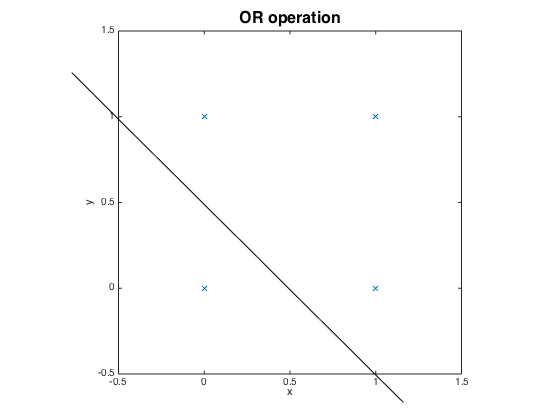
\includegraphics[width=225px]{./images/q0_a_1.png}
	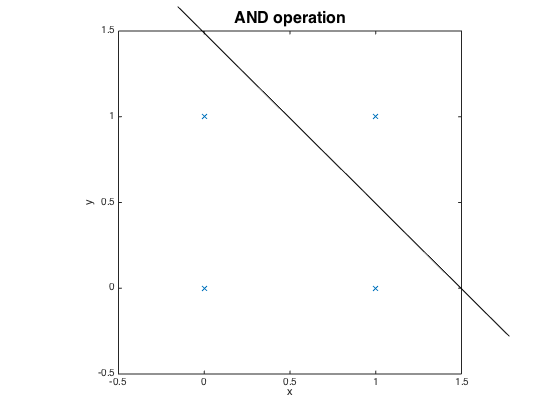
\includegraphics[width=225px]{./images/q0_a_2.png}\\
	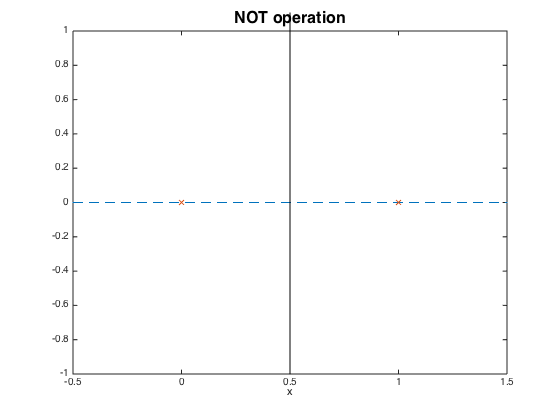
\includegraphics[width=225px]{./images/q0_a_3.png}
	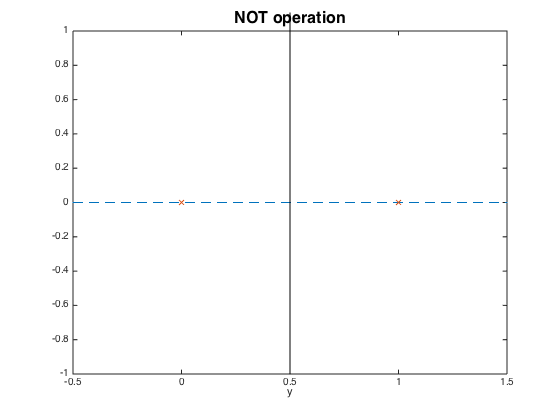
\includegraphics[width=225px]{./images/q0_a_4.png}\\
	For the OR operation, since there is a single line that can separate (0,0) from the other points such that (0,0) has class 0 while the other points have class 1, it can be computed using a single-layer linear classifier.\\ \\
For the AND operation, since there is a single line that can separate (1,1) from the other points such that (1,1) has class 1 while the other points have class 0, it can be computed using a single-layer linear classifier.\\ \\
For the NOT operation, we show that a linear classifier can be used to separate two points on a single axis.
\\
\\
	\textbf{b)}\\
$(x \lor y)$: $h_1(x,y) = \theta(x + y - 0.5)$\\
$\lnot (x \land y)$: $h_2(x,y) = \theta(-0.5 x - 0.5 y + .7)$\\
$(x \land y)$: $h_3(x,y) = \theta(0.5 x + 0.5y - 0.7)$
\end{homeworkProblem}

\pagebreak

\begin{homeworkProblem}
    \textbf{Solution}\\
	\textbf{a)}
\begin{align*}
	\frac{\delta J(\theta)}{\delta \theta} &= \hat{y} - y &&\text{from assignment 1}\\
	\frac{\delta \theta}{\delta U} &= h && \theta = Uh+b_2\\
	\frac{\delta J}{\delta U} &= \frac{\delta J(\theta)}{\theta} \frac{\delta \theta}{\delta U} = (\hat{y} - y) h\\
	\\
	\frac{\delta \theta}{\delta b_2} &= 1\\
	\frac{\delta J}{\delta b_2} &= (\hat{y} - y) \vec{1}\\
	\\
	\frac{\delta \theta}{\delta h} &= U\\
	\frac{\delta J}{\delta h} &= \frac{\delta J}{\delta \theta} \frac{\delta \theta}{\delta h} = (\hat{y} - y) U\\
	\\
	tanh'(z) &= \frac{\delta}{\delta z} sinh(z)/cosh(z)\\
	&= (cosh(z) \frac{\delta}{\delta z} sinh(z) - sinh(z) \frac{\delta}{\delta z} cosh(z)) / cosh^2(z)\\
	&= (cosh(z) cosh(z) - sinh(z) sinh(z)) / cosh^2(z)\\
	&= 1-tanh^2(z) \\
	h &= tanh(Wx^{(t)} + b_1)\\
	\frac{\delta h}{\delta W} &= tanh'(Wx^{(t)} + b_1) x^{(t)}\\
	\frac{\delta J}{\delta W} &= \frac{\delta J}{\delta h} \frac{\delta h}{\delta W} = ((\hat{y} - y) U) (tanh'(Wx^{(t)} + b_1) x^{(t)})\\
	\\
	\frac{\delta h}{\delta b_1} &= tanh'(Wx^{(t)} + b_1)\\
	\frac{\delta J}{\delta b_1} &= \frac{\delta J}{\delta h} \frac{\delta h}{\delta b_1} = ((\hat{y} - y) U) (tanh'(Wx^{(t)} + b_1))\\
	\\
	\frac{\delta h_i}{\delta L_k} &= \frac{\delta}{\delta L_k} (tanh(W_i x^{(t)} + b_{1,i}))\\
		&= tanh'(W_ix^{(t)} + b_{1,i}) \frac{\delta}{\delta L_k} (\sum_{j}W_{ij} x^{(t)}_j)\\
		&= tanh'(W_ix^{(t)} + b_{1,i}) W_{ik}\\
	\frac{\delta J}{\delta L_k} &= \frac{\delta J}{\delta h_i} \frac{\delta h_i}{\delta L_k} = ((\hat{y}_i - y_i)U_i)(tanh'(W_i x^{(t)} + b_{1,i}) W_{ik})
\end{align*}\\
\\
	\textbf{b)}
	\begin{align*}
		\frac{\delta J_{reg}}{\delta U} &= \lambda \sum_{i' j'} U_{i'j'}\\
		\frac{\delta J_{reg}}{\delta W} &= \lambda \sum_{ij} W_{ij}\\
		\frac{\delta J_{full}}{\delta U} &= \frac{\delta J}{\delta U} + \frac{\delta J_{reg}}{\delta U} = (\hat{y} - y)h + \lambda \sum_{i'j'} U_{i'j'}\\
		\frac{\delta J_{full}}{\delta W} &= \frac{\delta J}{\delta W} + \frac{\delta J_{reg}}{\delta W} = (\hat{y} - y)h + \lambda \sum_{ij} W_{ij}\\
	\\
	\frac{\delta J_{reg}}{\delta \theta} &= \frac{\delta J_{reg}}{\delta b_2} = \frac{\delta J_{reg}}{\delta b_1} = \frac{\delta J_{reg}}{\delta L_i} = 0\\
	\frac{\delta J_{full}}{\delta b_2} &= \frac{\delta J}{\delta b_2}\\
	\frac{\delta J_{full}}{\delta b_1} &= \frac{\delta J}{\delta b_1}\\
	\frac{\delta J_{full}}{\delta L_i} &= \frac{\delta J}{\delta L_i}
	\end{align*}
\\
\textbf{d)} I started with very coarse tuning of the hyperparameters and found that the given hyperparameters were already performing fairly well. I then did finer hyperparameter tuning around the given values, starting first with learning rate and regularization strength. Subsequently, I tuned the window size followed by the training schedule and minibatch size.\\ 
My best performing model has a F-1 score of \textbf{80.10\%} using minibatch gradient descent with batch size 7, window size 5, regularization strenght 0.001 and learning rate of 0.01.\\
\\
\textbf{e)}
\\
\centerline{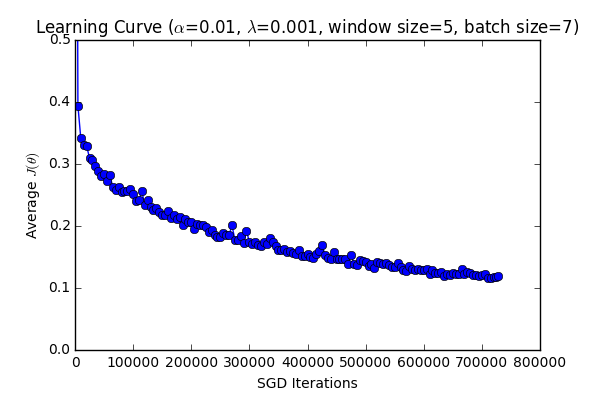
\includegraphics[width=300px]{./images/q2e.png}}\\
\centerline{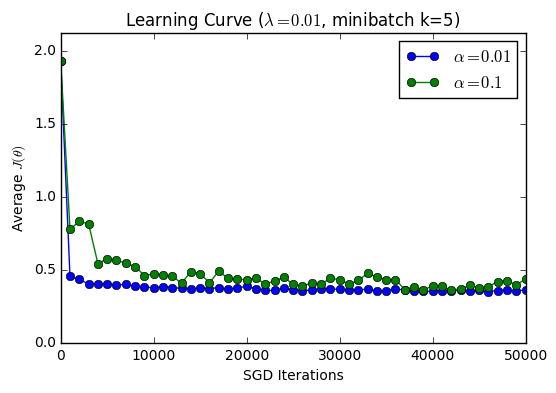
\includegraphics[width=300px]{./images/q2e_2.png}}\\
When the model learns too quickly (i.e. when $\alpha=0.1$), the cost moves up and down more during the training process and tends to decrease more slowly. The model also does not converge properly within the given number of iterations. Intuitively, this is because the steps taken during each gradient descent are large and the model is less likely to reach an optimum.\\
\\
\textbf{f)}
\\
The performance of my model on the dev set is as follows:
\begin{verbatim}
=== Performance (omitting 'O' class) ===
Mean precision:  83.62%
Mean recall:     77.14%
Mean F1:         80.10%
\end{verbatim}
\textbf{1.1)a)}
\begin{verbatim}
Neuron 1
[0]: (0.460) recorded
[1]: (0.474) olympic
[2]: (0.463) apology
[3]: (0.483) outcome
[4]: (0.508) english
[5]: (0.592) open
[6]: (0.509) index
[7]: (0.498) australian
[8]: (0.488) prize
[9]: (0.619) cup
Neuron 3
[0]: (0.980) achievement
[1]: (0.983) broadcast
[2]: (0.988) radio
[3]: (1.009) quiz
[4]: (1.029) arithmetic
[5]: (1.082) instruction
[6]: (1.052) electronic
[7]: (1.148) educational
[8]: (1.072) curriculum
[9]: (1.093) select
Neuron 4
[0]: (0.825) korea
[1]: (0.866) continually
[2]: (0.874) dock
[3]: (0.898) partially
[4]: (0.871) china
[5]: (0.978) indirectly
[6]: (1.040) thereby
[7]: (1.085) temporarily
[8]: (1.003) behalf
[9]: (1.015) permanently
Neuron 6
[0]: (0.407) estimated
[1]: (0.414) english
[2]: (0.417) recorded
[3]: (0.418) apology
[4]: (0.427) prize
[5]: (0.427) outcome
[6]: (0.438) example
[7]: (0.491) open
[8]: (0.445) index
[9]: (0.501) cup
Neuron 8
[0]: (1.319) 'd
[1]: (1.328) worse
[2]: (1.363) thereafter
[3]: (1.367) nothing
[4]: (1.393) sadly
[5]: (1.555) unfortunately
[6]: (1.584) there
[7]: (1.398) aside
[8]: (1.521) afterwards
[9]: (1.828) suddenly
\end{verbatim}
Neurons in this model appear to have learned words that have 1) similar semantic relationship (e.g. Neuron 1: olympic, cup, prize, open) or 2) similar structure (e.g. Neuron 4 has adverbs: continually, partially, indirectly, temporarily).\\
\\
\textbf{1.1)b)}
\begin{verbatim}
Output neuron 1: LOC
[0]: (0.005) japan
[1]: (0.005) russia
[2]: (0.005) korea
[3]: (0.008) england
[4]: (0.005) mexico
[5]: (0.006) pakistan
[6]: (0.005) germany
[7]: (0.007) china
[8]: (0.007) italy
[9]: (0.005) norway

Output neuron 2: MISC
[0]: (0.003) belgian
[1]: (0.003) german
[2]: (0.003) english
[3]: (0.003) turkish
[4]: (0.004) brazilian
[5]: (0.004) italian
[6]: (0.005) open
[7]: (0.004) danish
[8]: (0.005) cup
[9]: (0.004) israeli

Output neuron 3: ORG
[0]: (0.001) colleges
[1]: (0.002) computing
[2]: (0.002) curriculum
[3]: (0.002) reuters
[4]: (0.002) libraries
[5]: (0.002) commons
[6]: (0.002) corp
[7]: (0.003) &
[8]: (0.002) microsoft
[9]: (0.002) inc

Output neuron 4: PER
[0]: (0.004) miller
[1]: (0.006) carter
[2]: (0.005) wilson
[3]: (0.007) clinton
[4]: (0.009) thompson
[5]: (0.004) jim
[6]: (0.004) martin
[7]: (0.005) scott
[8]: (0.005) pat
[9]: (0.006) jr.
\end{verbatim}
The model appear to have correctly learned the named entities. For instance, the output neuron corresponding to the LOC class activates for names of countries, and the output neuron corresponding to the PER class activates (mostly) for the names of people.\\
\\ 
\textbf{1.1)c)}
\begin{verbatim}
Output neuron 1: LOC
[0]: (0.000) surrounding
[1]: (0.000) left
[2]: (0.001) reaches
[3]: (0.000) outside
[4]: (0.000) located
[5]: (0.000) at
[6]: (0.001) near
[7]: (0.000) visiting
[8]: (0.000) inhabited
[9]: (0.000) in

Output neuron 2: MISC
[0]: (0.000) modern
[1]: (0.000) existence
[2]: (0.000) tour
[3]: (0.000) ancient
[4]: (0.000) medieval
[5]: (0.000) world
[6]: (0.000) major
[7]: (0.000) million
[8]: (0.000) series
[9]: (0.000) league

Output neuron 3: ORG
[0]: (0.000) charity
[1]: (0.000) oracle
[2]: (0.000) communications
[3]: (0.000) grove
[4]: (0.001) &
[5]: (0.001) corporation
[6]: (0.001) v
[7]: (0.001) inc.
[8]: (0.001) workshops
[9]: (0.001) enterprise

Output neuron 4: PER
[0]: (0.001) aunt
[1]: (0.001) jr.
[2]: (0.002) dejected
[3]: (0.001) mike
[4]: (0.002) don
[5]: (0.002) pat
[6]: (0.002) mate
[7]: (0.001) m.
[8]: (0.002) peter
[9]: (0.001) ode
\end{verbatim}
Many of these output neurons activate for words that tend to precede those in (c). For instance, many of the preceding words in LOC are prepositions.\\
\\
\end{homeworkProblem}
\pagebreak
\begin{homeworkProblem}
	\textbf{Solution}\\
	\textbf{a)}
	\begin{align*}
		J^{(t)}(\theta) &= -\sum_{j=1}^{\vert V \vert} y_j^{(t)} log_2 \hat{y}_j^{(t)} &&\text{$y^{(t)}$ is one-hot vector}\\
		&= - log_2 \hat{y}_k^{(t)} &&\text{let $k$ be the index of the target word}\\
		PP^{(t)} (\hat{y}^{(t)}, y^{(t)}) &= 2^{J(\theta)}\\
		&= 2^{-log_2 \hat{y}_k^{(t)}}\\
		&= (\hat{y}_k^{(t)})^{-1}\\
		&= \frac{1}{\hat{y}_k^{(t)}}\\
		&= \frac{1}{\sum_{j=1}^{\vert V \vert} y_j^{(t)} \cdot \hat{y}_j^{(t)}}
	\end{align*}
If we express the loss as the (arithmetic) mean cross-entropy loss over the dataset of size T:
	\begin{align*}
		J &= -\frac{1}{T} \sum_{t=1}^T \sum_{j=1}^{\vert V \vert} y_{t,j} log_2 \hat{y}_{t,j}\\
		&= -\frac{1}{T} \sum_{t=1}^T log_2 \hat{y}_{t,k} &&\text{where $k$ is the index of the target word}\\
		PP(\hat{y}^{(t)}, y^{(t)}) &= 2^{-\frac{1}{T} \sum_{t=1}^T log_2 \hat{y}_{t,k}}\\
		&= (2^{\sum_{t=1}^T log_2 \hat{y}_{t,k}})^{-\frac{1}{T}}\\
		&= (\prod_{t=1}^T \hat{y}_{t,k})^{-\frac{1}{T}}\\
		&= \sqrt[T]{\frac{1}{\prod_{t=1}^T \hat{y}_{t,k}}}
	\end{align*}
Minimizing $J$, i.e. the arithmetic mean cross-entropy loss, is equivalent to minimizing $PP$, i.e. the geometric mean perplexity.\\
\\
	\textbf{b)}
	\begin{align*}
		\frac{\delta J^{(t)}(\theta)}{\delta \theta} &= \hat{y}^{(t)} - y^{(t)}\\
		\frac{\delta \theta}{\delta U} &= h^{(t)} &\theta = Uh^{(t)}\\ 
		\frac{\delta J^{(t)}}{\delta U} &= \frac{\delta J^{(t)}}{\delta \theta} \cdot \frac{\delta \theta}{\delta U} = (\hat{y}^{(t)} - y^{(t)})h^{(t)}\\
		\\
		\frac{\delta h^{(t)}}{\delta H} &= sigmoid'(H h^{(t-1)} + Lx^{(t)}) \cdot h^{(t-1)} &h^{(t)} = sigmoid(Hh^{(t-1)} + Lx^{(t)})\\
		\frac{\delta \theta}{\delta h^{(t)}} &= U\\
		\frac{\delta J^{(t)}}{\delta h^{(t)}} &= \frac{\delta J^{(t)}}{\delta \theta} \cdot \frac{\delta \theta}{\delta h^{(t)}} = (\hat{y}^{(t)} - y^{(t)}) U\\
		\frac{\delta J^{(t)}}{\delta H} &= \frac{\delta J^{(t)}}{\delta h^{(t)}} \cdot \frac{\delta h^{(t)}}{\delta H} = ((\hat{y}^{(t)} - y^{(t)}) U)(sigmoid'(Hh^{(t-1)} + Lx^{(t)}) h^{(t-1)}\\
		\\
		\frac{\delta h^{(t)}}{\delta (L_{x^{(t)}})_j} &= sigmoid'(Hh^{(t-1)} + Lx^{(t)})_j\\
		\frac{\delta J^{(t)}}{\delta (L_{x^{(t)}})_j} &= \frac{\delta J^{(t)}}{\delta h^{(t)}} \cdot \frac{\delta h^{(t)}}{\delta (L_{x^{(t)}})_j} = ((\hat{y}^{(t)} - y^{(t)}) U )(sigmoid'(H h^{(t-1)} + L x^{(t)})_j)\\
		\\
		\frac{\delta h^{(t)}}{\delta h^{(t-1)}} &= sigmoid'(Hh^{(t-1)} + Lx^{(t)}) H\\
		\frac{\delta J^{(t)}}{\delta h^{(t-1)}} &= \frac{\delta J^{(t)}}{\delta h^{(t)}}\frac{\delta h^{(t)}}{\delta h^{(t-1)}} = ((\hat{y}^{(t)} - y^{(t)}) U)(sigmoid'(Hh^{(t-1)}+Lx^{(t)}) H)\\
	\end{align*}
\\
	\textbf{(c)}\\
	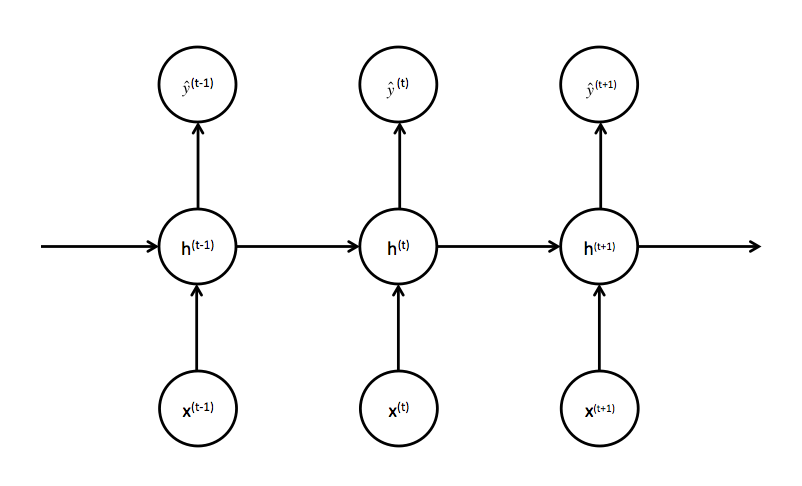
\includegraphics[width=300px]{./images/q2c.png}\\
	\begin{align*}
		\frac{\delta J^{(t)}}{\delta (L_{x^{(t-1)}})_j} &= \frac{\delta h^{(t-1)}}{\delta (L_{x^{(t-1)}})} \frac{\delta h^{(t)}}{\delta h^{(t-1)}} \frac{\delta J^{(t)}}{\delta h^{(t)}}\\
		&= sigmoid'(Hh^{(t-2)} + Lx^{(t-1)})_j sigmoid'(Hh^{(t-1)} + Lx^{(t)})H (\hat{y}^{(t)} - y^{(t)}) U\\
		&= \frac{\delta J^{(t)}}{\delta (L_{x^{(t)}})_j} sigmoid'(Hh^{(t-2)} + Lx^{(t-1)})H\\
		&= \delta^{(t)} sigmoid'(Hh^{(t-2)} + Lx^{(t-1)})H\\
		\\
		h^{(t-1)} &= sigmoid(Hh^{(t-2)} + Lx^{(t-1)})\\
		\frac{\delta h^{(t-1)}}{\delta H} &= sigmoid'(Hh^{(t-2)} + Lx^{(t-1)}) h^{(t-2)}\\
		\frac{\delta h^{(t)}}{\delta H} &=\frac{\delta h^{(t)}}{\delta h^{(t-1)}} \frac{\delta h^{(t-1)}}{\delta H}\\
		&= (sigmoid'(Hh^{(t-1)} + Lx^{(t)}) H)(sigmoid'(Hh^{(t-2)} + Lx^{(t-1)}) h^{(t-2)})\\
		\frac{\delta J^{(t)}}{\delta H} \bigg|_{(t-1)} &= ((\hat{y}^{(t)} - y^{(t)})U)(sigmoid'(Hh^{(t-1)}+Lx^{(t)})H)(sigmoid'(Hh^{(t-2)}+Lx^{(t-1)})h^{(t-2)})\\
		&= \delta^{(t-1)} h^{(t-2)}
	\end{align*}
	\textbf{d)}\\
	For forward propagation, the matrix multiplications $Hh^{(h-1)}$, $Lx^{(t)}$ and $Uh^{(t)}$ take $D_h^3$, $D_h^2 \vert V\vert$, $\vert V \vert D_h$ operations respectively. $J^{(t)}$ requires summing over $\vert V\vert$. Therefore, forward propagation has $O(\vert V\vert^2 D_h^2)$ complexity.\\
	For backpropagation, the largest operation is the matrix multiplication involving $D_h^2 \vert V \vert$. As such, backpropagation for a single time step is $O(D_h^2 \vert V \vert)$ and backpropagation for $\tau$ time steps is $O(\tau D_h^2 \vert V \vert)$.\\
The slowest step is in the forward propagation.\\
	\\
	\textbf{f)} The best hyperparameters used are:
	\begin{itemize}
		\item Dimension of hidden layer: 100
		\item Learning rate: 0.1
		\item Backprop timesteps: 2
		\item Minibatch size: 5
	\end{itemize}
	The model was trained for 1 epoch of the full training set and gave an unadjusted perplexity of 74.583 and adjusted perplexity of 119.584.\\
	\\
	\textbf{g)}
	\begin{verbatim}
<s> UUUNKKK , although it 's UUUNKKK kept UUUNKKK under `` a major marketing UUUNKKK for it 
had a UUUNKKK partnership has , including wall executive officer of about DGDGDGDG , and 
they would still UUUNKKK the managing stock as a UUUNKKK UUUNKKK , is big exchange took 
UUUNKKK called through damage on the UUUNKKK of a third-quarter prime charges , mixed 
equipment UUUNKKK time to UUUNKKK the UUUNKKK of october services , done win UUUNKKK 
development , it would been less , and that is UUUNKKK fourth estimate UUUNKKK , they can 
a UUUNKKK with a UUUNKKK about the UUUNKKK

<s> and the ad can begin early manufacturing most tax oil newspaper saw even UUUNKKK to 
he will be clearly '' there </s>

<s> the court reached UUUNKKK majority next are release in the acquisition of UUUNKKK said , 
despite the UUUNKKK from fixed japanese stock restructuring , he have paying UUUNKKK financial 
of a year earlier , compared and UUUNKKK UUUNKKK , UUUNKKK , to remained oct. DG higher time , 
economist they has last UUUNKKK UUUNKKK . </s>
	\end{verbatim}
\end{homeworkProblem}
\end{document}
